% Chapter 4

% variables
\newcommand{\pdirfour}{chapters/plots/chapter4}

\chapter{Results} % Main chapter title

\label{chapter4} % For referencing the chapter elsewhere, use \ref{Chapter1}

In this chapter, we summarize the results of the NA64 experiment to this date, which include all the runs up to 2018 \cite{Banerjee:2020fue,Banerjee:2019hmi,NA64:2019imj,na64-prd,Banerjee:2018vgk,Banerjee:2016tad}. In the previous chapter, we estimated the background, defined the selection criteria, and computed the signal yield. Now all is left to do is to un-blind the signal region and apply our selection criteria to the full sample, and count the number of events in the signal region that we defined. No event was found in the signal region in all analyses performed. This leaves us with the task of rejecting a set of hypothesis $\dmhypo$ that is not compatible with the data collected. This is done using the modified frequentist approach to compute the confidence level, taking the profile likelihood as test statistic in the asymptotic approximation \cite{Read_2002,JUNK1999435,Cowan:2010js}. This technique is summarized in Appendix.\ref{AppendixE}, and uses a representative data set provided by the Monte Carlo (also called Asimov data set) to obtain the median experimental sensitivity and its uncertainty. In this chapter, we will present the results in two different planes. First, in Sec.\ref{ch4:sec:exclusion-limits}, we will show in the $\dmplane$ plane which models are rejected by our searches, and compare the results to constraints from other measurements. This will be done for data of both visible and invisible mode, and we will briefly discuss the implication for the $\DMX$-anomaly discussed in Sec.\ref{ch1:sec:dm-u1model-motivations-x17}. Results on ALPs and light scalar particles following a new analysis of the invisible mode data are also reported, presented in the $(g_{a\gamma \gamma};m_a)$ plane. Finally, in Sec.\ref{ch4:sec:exclusion-limits-y}, the results of the invisible mode are also presented in the $\dmyplane$ plane introduced in chapter \ref{chapter1}, to show our sensitivity for the region of parameter space compatible with the observed relic density in the freeze-out framework.

%----------------------------------------------------------------------------------------

\section{Exclusion limits in the $\dmplane$ plane}
\label{ch4:sec:exclusion-limits}

To date, no event has been recorded in the signal region defined for the invisible/visible mode setup. The results of all analyses are shown in Fig.\ref{fig:exclusion-dmplane}. The curves were obtained using the MC simulation to build Asimov dataset for different hypothesis $\dmhypo$ used to compute the signal yield as described in the previous chapter. The single data points are then used to build a full curve using a smooth Bézier interpolation.

In the case of invisible mode, the main interest of the scientific community was if the $\DM$ can be a viable explanation for the anomalous magnetic moment of the muon $a_{\mu}$. At present, the data collected by NA64 rejects the hypothesis that the deviation of $a_{\mu}$ can be attributed to the $\DM$. This was confirmed independently by the BABAR experiment, which was the first one to publish a paper excluding completely this region of the parameter space \cite{PhysRevLett.119.131804}.

One more case under consideration was the one of ALPs and light scalar particles that couples to photons via the Primakoff effect. For this search, data from the invisible mode setup are used and the signal box is changed slightly: now only the first HCAL module is used as VETO, and the second and third modules are allowed to contain all the energy missing from the ECAL, as the ALPs (or light scalar) particle will decay $a(s) \to \gamma \gamma$ similarly to the visible mode. This search presents background slightly different from the one of the invisible mode, which was studied in \cite{Banerjee:2020fue}. The results are presented in Fig.\ref{fig:exclusion-dmplane-alps}

An interesting feature is the different shape of the exclusion curve in the two modes. In the case of the invisible mode, the production of $\DM$ is sufficient for the experiment to detect it\footnote{Providing the event can pass all selection criteria, whose efficiency depends only weakly on the precise $\dmhypo$.}, so only the cross-section is limiting our signal yield. Looking at Eq.\ref{eq:dm-rate} back in chapter 1, we see that the rate depends quadratically on both parameters of the theory. This leads to a curve similar to a parabola in the log-log plane, with large mass and low coupling harder to probe due to the lower value of the cross-section. In the visible mode parameter space, on the other hand, we observe that a part of the parameter space that is not probed even though the coupling $\epsilon$ is high and the mass relatively small. The reason, as detailed in Sec.\ref{ch3:sec:vis-mode-tracking}, has to do with the detection efficiency of $\DMM$. A large coupling implies the production of a large number of $\DMM$, but we can see in Eq.\ref{eq:dm-rate-vis-limit} that the decay length is reduced. Since we can only detect decays that happen outside the target, we need to consider the exponential distribution of the decay only from the end of the dump. We proved back in chapter \ref{chapter1} that the number of events will be exponentially suppressed because of this effect, and increasing the number of events contributes therefore only logarithmically to the signal yield. The result can be observed in the plot: the exclusion region shows two regimes, one at $\epsilon < 10^{-4}$ dominated by the production of $\DMM$ that scales linearly with the EOTs accumulated and one at $\epsilon > 3 \times 10^{-4}$ dominated by the efficiency in detection that scales only logarithmically with them.

In the case of the visible mode, one has to be careful how to interpret the parameter space drawn for the $\DMX$. The line is only valid for a protophobic vector boson explanation, which we saw was only one of many possibilities in Sec.\ref{ch1:sec:dm-u1model-motivations-x17}. Also, it appears from the plot that the NA48 experiment already covers a relevant region for $\DMX$, but this not accurate. Because of its (alleged) protophobic nature, the $\DMX$ cannot be searched using the $\pi^0 \rightarrow \gamma \DM$ decay. This means those limit are only valid for the usual $\DM$ decaying visibly, and cannot be extended to a protophobic vector boson like for NA64. The $\DMX$ parameter space to date is excluded for $1.2 \times 10^{-4} \lesssim \epsilon \lesssim 6.8 \times 10^{-4}$ with the data collected in 2018. We saw in chapter \ref{chapter1} that to justify the $\DMX$-anomaly a coupling up to $\epsilon \simeq 1.4 \times 10^{-3}$ is allowed if the mediator is assumed to be a protophobic vector boson. This leaves a particularly difficult region of the parameter space left to explore. The final task of my Ph.D. was to contribute to the design of an experiment able to cover the region with a feasible amount of EOT. This new design is covered in Sec.\ref{ch5:sec:new-vismode-setup}.

\begin{figure}[tbh!]
  \centering
  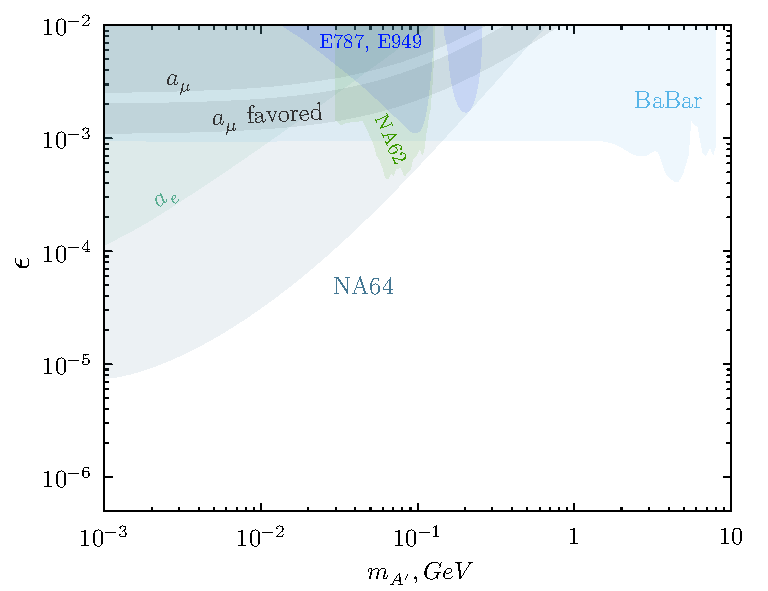
\includegraphics[width=0.45\textwidth,height=0.515\textwidth]{\pdirfour/exclusionInvisible.pdf}
  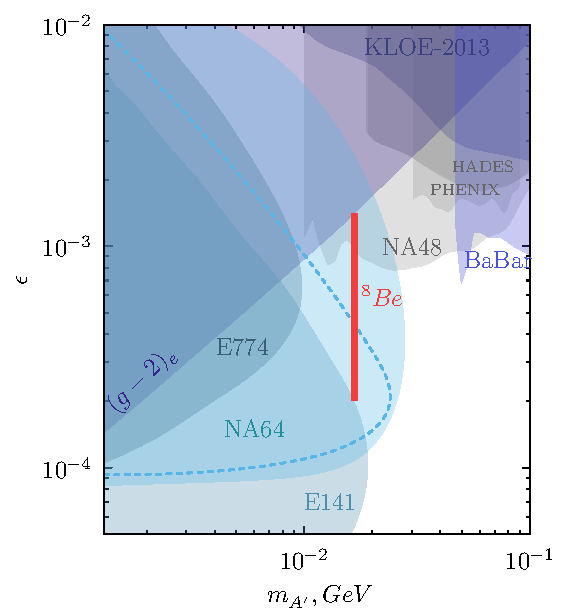
\includegraphics[width=0.45\textwidth,height=0.5\textwidth]{\pdirfour/exclusionVisible.pdf}
  \caption[Exclusion limits in the $\dmplane$]{The NA64 90\% exclusion region in the $\dmplane$ plane. The exclusion is shown for the data collected in the invisible mode setup (right) and visible mode setup (left), assuming the dominant decay is either invisible or visible respectively\cite{NA64:2019imj,Banerjee:2019hmi}. For the invisible mode, constraints from E787 and E949 \cite{PhysRevD.89.095006,Essig:2013vha},BABAR \cite{PhysRevLett.119.131804}, and recent NA62 results \cite{CortinaGil:2019nuo} are also shown, together with the muon $a_{\mu}$ favored area. For the visible mode, constraints from the experiments E774 \cite{PhysRevLett.67.2942}, E141 \cite{PhysRevLett.59.755}, BABAR \cite{babar1}, KLOE \cite{kloe2}, HADES \cite{hades}, PHENIX \cite{phenix}, NA48 \cite{na48} and bounds from the anomalous magnetic moment of the electron \cite{PhysRevD.89.095006} are shown. A blue dotted line shows the previous limit obtained with the analysis of the 2017 data. A thick red line shows the full parameter space that can justify the $\DMX$-anomaly \cite{PhysRevD.95.035017}, $2 \times 10^{4} < \epsilon< 1.4 \times 10^{-3}$. Currently, NA64 exclude coupling $\epsilon < 6.8 \times 10^{-4}$ for a $\DMX$ mass of 16.7 \mev.}
  \label{fig:exclusion-dmplane}
\end{figure}

\begin{figure}[bth!]
  \centering
  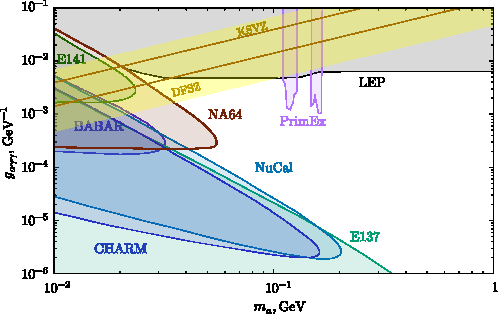
\includegraphics[width=0.7\textwidth]{\pdirfour/alps_new.pdf}
  \caption[Exclusion limits in the $(m_{a};g_{a \gamma \gamma})$ plane for ALPS and light scalar]{The 90\% exclusion limit for ALPS and light scalar particle obtained from the full dataset 2016-2018 in NA64 plotted in the $(m_{a};g_{a \gamma \gamma})$ plane. The yellow band represents the parameter space for the benchmark DFSZ \cite{DINE1981199} and KVSZ \cite{PhysRevLett.43.103} models. Constraint from BABAR \cite{Dolan:2017osp}, E137 \cite{e137}, E141 \cite{blum}, LEP , and PrimEx \cite{PhysRevLett.123.071801} experiments, as well as limits from CHARM \cite{BERGSMA1985458} and NuCal \cite{Dobrich:2019dxc} are also shown.}
  \label{fig:exclusion-dmplane-alps}
\end{figure}

\newpage

\section{Exclusion limits in the $\dmyplane$ plane}
\label{ch4:sec:exclusion-limits-y}

Our results have also an impact in the broader framework of cosmological dark matter. As detailed in chapter \ref{chapter1}, various dark sector models motivate sub-$\gev$ scalar and Majorana or pseudo-Dirac fermium Dark Matter coupled to dark photons \cite{battaglieri2017cosmic}. We can use the requirement of the thermal freeze out of DM annihilation into visible matter to derive a relation between the interesting parameters of the model \cite{na64-prd}:

\begin{equation}
  \label{eq:ad-freeze-out}
  \alpha_D \simeq 0.02 f\left(\frac{10^-3}{\epsilon}\right)^2\left(\frac{m_{\DM}}{100 \mev}\right)^2\left(\frac{10 \mev}{m_{\chi}}\right)^2
\end{equation}

Where we define $\alpha_d = e^2_D/4\pi$, $f\lesssim 10$ for a scalar \cite{deNiverville:2011it}, and $f\lesssim 1$ for a fermion \cite{PhysRevD.91.094026}. Dark Matters models can be classified by the spin and masses of the mediator. Here we consider the vector case that is relevant to us, and we remind that scalar mediators are restricted by the non-observation of rare B-meson decay \cite{battaglieri2017cosmic}. Hence, we convert our constraint in the $\dmplane$ in constraint on the $\dmyplane$ plane using Eq.\ref{eq:dmplane-y-dp}, and assuming different values of $\alpha_D$/$m_{\chi}$ we exclude hypothesis not compatible with the data collected. In Fig.\ref{fig:dm-alpha-excl} the results are presented in this form, assuming $m_{\DM} = 3m_{\chi}$ and taking $\alpha_D=0.1$ and $\alpha=0.5$ as benchmark values for the comparison, which are values compatible with the derivation of running coupling in the dark sector of \cite{Davoudiasl:2015hxa}. We used $f=0.25$ for the case of pseudo-Dirac fermion and f=3 for the case of Majorana. It should also be noted that for the case of smaller $\alpha_D$ the experimental bound shown would be more restrictive, as the yield in NA64 depends on just $\epsilon^2$ and not $\epsilon^4 \alpha_D$ like many beam-dump searches. In conclusion, the results are promising, the region compatible with the observed relic density under the assumption of a freeze-out mechanism is still not in the NA64 experimental sensitivity. A larger number of EOT needs to be collected to probe that region of parameter space.

\begin{figure}[bth!]
  \centering
  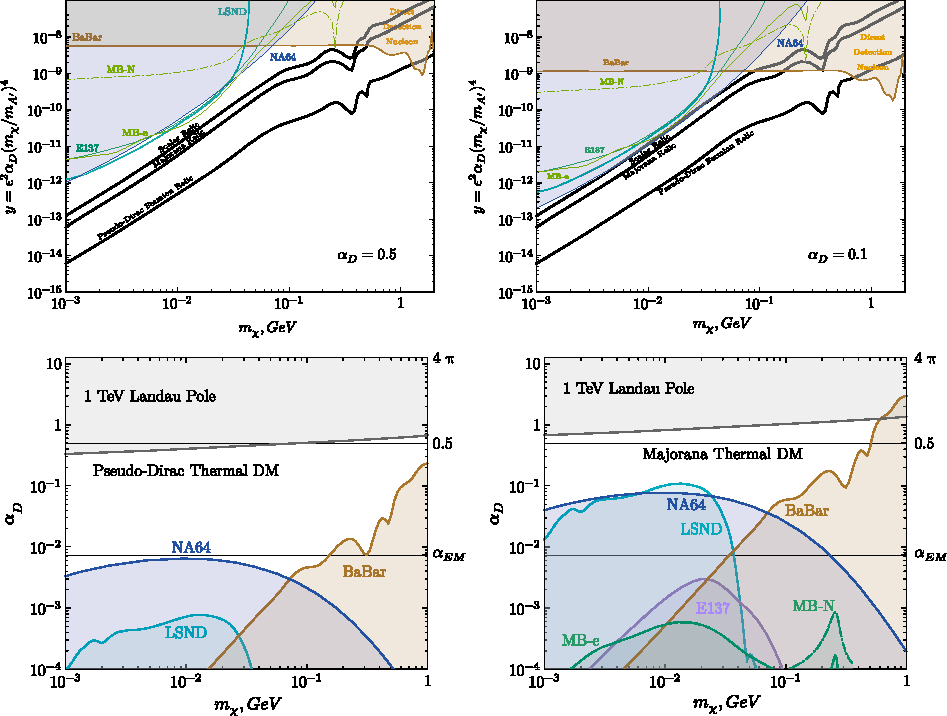
\includegraphics[width=\textwidth]{\pdirfour/tldra-complete.pdf}
  \caption[Exclusion limit in the $dmyplane$ for scalr, pseudo-Dirac and Majorana type of light Dark Matter]{The top rows show the NA64 limits in the $\dmyplane$ plane obtained for $\alpha_D = 0.5$ (left panel) and $\alpha_D = 0.1$ (right panel) from the full 2016-2018 data set. The bottom rows shows the same constraint in the $\dmaplane$ for the pseudo-Dirac (left panel) and Majorana (right panel) Dark matter. The limits are shown in comparison with the bounds obtained from the results of the LNSD \cite{deNiverville:2011it}, E137 \cite{e137}, MiniBooNE \cite{Aguilar-Arevalo:2018wea}, BABAR \cite{babar1} and direct detection experiments \cite{Essig:2012yx}. The favored parameters to account for the observed relic DM density for the scalar, pseudo-Dirac and Majorana type of light DM are shown as the lowest solid line in top plots \cite{Berlin:2018bsc}.}
  \label{fig:dm-alpha-excl}
\end{figure}
%%% Local Variables:
%%% mode: latex
%%% TeX-master: "../PhDthesis"
%%% End:
